\documentclass[12pt, a4paper]{article}
\usepackage[romanian]{babel}
\usepackage{fancyhdr}
\usepackage{graphicx}
\usepackage{amsmath}
\usepackage{multirow}
\usepackage{array}

\renewcommand{\arraystretch}{1.5}

\DeclareGraphicsExtensions{.pdf,.png}

\title{\centering{Oscilații armonice\\ cu forța de rezistență a aerului}}
\author{Negru Mihai}
\date{Martie 2022}

\pagestyle{fancy}
\fancyhf{}
\rhead{Negru Mihai}
\lhead{Universitatea Politehnica din București}
\cfoot{\thepage}

\begin{document}

\maketitle
\newpage
\tableofcontents{}
\newpage
\section{Prezentarea lucrării}
\subsection{Tematica lucrării}
\hspace{0.4cm}În această lucreare vom aborda un fenomen fizic mecanic cunoscut de orice persoană, pentru a 
întări cunoștințele în rezolvarea ecuațiilor diferențiale cu coeficienți reali prin metode analitice dar și prin metode numerice. Totodată prin această lucrare vă veți dezvolta simțul fizic pentru perceperea lucrurilor și fenomenelor înconjurătoare, veți observa în deaproape aplicațiile ecuațiilor diferențiale în viața de zi cu zi, veți face distincția dintre mai multe metode de rezolvare și abordare a problemelor din aceiași clasă cu problema prezentată în lucrare.
\subsection{Subiectul lucrării}
\hspace{0.4cm}În mare parte lucrarea se axează pe înțelegerea cititorului a metodelor de rezolvare, să poată face diferența dintre rezolvarea unei metode analitice și cea numerice, să poată decide dacă se merită o rezolvare analitică, lungă, anevoioasă, cu posibile erori de calcul sau pur și simplu neatenție, versus o metodă care pentru o anumită condiție, rezolvă ecuația diferențială cu eroare de marjă aproximativ nesimnificativă.Totodată pentru unele ecuații sau în jurul unor alte condiții este mai bine să folosim o metodă analitică a problemei, totuți să nu uităm că sistemele de calcul (calculatoarele) nu pot păstra o infinitate de zerouri în baza lor de date, astfel și aceste sisteme fac niște aproximări și atunci se pune întrebarea de ce să nu rezolvăm o problemă mai simplu, unde sistemul de calcul face toată rutina pentru tine.  
\subsection{Abordarea lucrării}
%\hspace{0.4cm}Lucrarea este scrisă în 5 capitole.Primul capitol descrie fenomenul fizic în limbaj matematic, al doilea capitol prezintă o abordare matematică precisă pentru rezolvarea ecuației diferențiale cu metode analitice cunoscute și o metodă numită transformarea Laplace.Mai apoi vom încerca rezolvarea ecuației diferențiale prin renumita metodă a lui Euler pentru aproximarea soluției ecuației diferențiale.Ultimele capitole se axează pe diferența și compararea dintre rezolvarea metodelor analitice și numerice, încheindu-se cu o concluzie de rigoare.Pentru a putea rezolva numeric vom avea nevoie de un program puternic de calcul matematic specializat pe operații vectoriale, astfel problema va fi rezolvată în Matlab R2021. (În caz că nu dispuneți de licență Matlab puteți folosi versiunea free Octave).
\begin{description}
\item [Inceput:] Lucrarea este scrisă în 5 capitole.Primul capitol descrie fenomenul fizic în limbaj matematic, al doilea capitol prezintă o abordare matematică precisă pentru rezolvarea ecuației diferențiale cu metode analitice cunoscute și o metodă numită transformarea Laplace.
\item [Analiză:] Mai apoi vom încerca rezolvarea ecuației diferențiale prin renumita metodă a lui Euler pentru aproximarea soluției ecuației diferențiale.
\item [Final:] Ultimele capitole se axează pe diferența și compararea dintre rezolvarea metodelor analitice și numerice, încheindu-se cu o concluzie de rigoare.
\end{description}

\section{Fenomenul Fizic}
\begin{figure}[h]
    \centering
    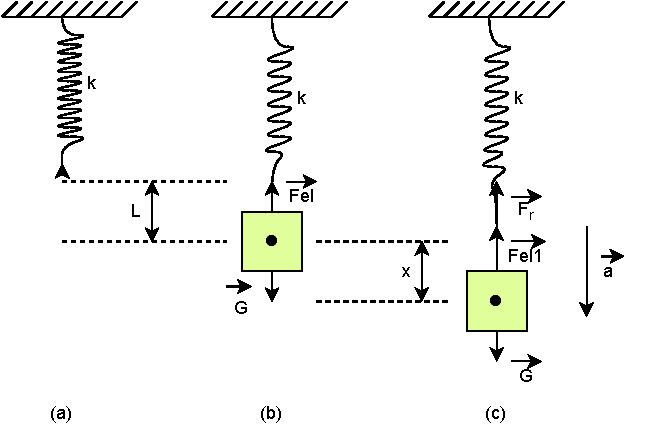
\includegraphics[width=\linewidth, scale=5]{Oscilatii}
    \caption{Oscilații armonice}
    \label{fig:oscilatii}
\end{figure}

\subsection{Descrierea fenomenului fizic}
\hspace{0.4cm}După cum putem observa în figura \ref{fig:oscilatii} (a) avem un resort ce se atârnă de un stativ necuplat cu nici o masă care are constanta de elasticitate $k$. În figura \ref{fig:oscilatii} (b) vom atârna de resort o greutate de masă $m$ și acest corp va crea o deformație egală cu $l$, iar apoi imprimăm o forță ceea ce va conduce la o nouă deformație egală cu $x$. În cele ce urmează vom încerca să aflăm o relație ce leagă deformația nou imprimată $x$ de sistemul descris mai sus, iar mai apoi vom încerca să aflăm dependența deformației în funcție de timp $x(t)$ prin metode de bază și metode avansate.
\newpage
\subsection{Abordarea matematică a fenomenului}
\hspace{0.6cm}În figura \ref{fig:oscilatii} (b) corpul se află într-o poziție de echilibru și atunci scriind legea a II-a al lui Newton obținem $\overrightarrow{F_{el}}\;+\;\overrightarrow{G} = 0$, iar din figura \ref{fig:oscilatii} (c) obținem relația $\overrightarrow{F_{el1}}\;+\overrightarrow{F_{r}}\;+\;\overrightarrow{G} = m\overrightarrow{a}$, atunci lucrul nostru de ingineri devotați este să rezolvăm sistemul:

\begin{equation}
\left\{
    \begin{array}{lr}
        \overrightarrow{F_{el}}\;+\;\overrightarrow{G} = 0\\
        \overrightarrow{F_{el1}}\;+\overrightarrow{F_{r}}\;+\;\overrightarrow{G} = m\overrightarrow{a}
    \end{array}
\right.
\end{equation}

Vom proiecta pe axa paralelă cu accelerația și orientată la fel ca accelerația:

\begin{equation}
\left\{
    \begin{array}{lr}
        -F_{el}\;+\;G = 0\\
        -F_{el1}\;-F_{r}\;+\;G = ma
    \end{array}
\right.
\end{equation}

Cum forța elastică în cazul (b), conform legii lui Hooke este $F_{el} = kl$ și în cazul (c) $F_{el1} = k(x\;+\;l)$, iar forța de rezistență a aerului $F_{r} \sim v$, înseamnă că $F_{r} = \beta v$, unde $\beta$ este un coeficient real. Atunci sistemul anterior rezultă:

\begin{equation}
\left\{
    \begin{array}{lr}
        -kl\;+\;mg = 0\\
        -k(x\;+\;l)\;-\;\beta v\;+\;mg = ma
    \end{array}
\right.
\end{equation}

Combinând cele două ecuații, trecând toțimembri în partea dreaptă și împărțind la masa corpului $m$ care este diferită de zero, oricare ar fi corpul suspendat, rezultă ecuația:

\begin{equation}
    a\;+\;\frac{\beta}{m}v\;+\;\frac{k}{m}x = 0
\end{equation}

Trecând accelerația, viteza în derivate ale distanței față de timp obținem următorul rezultat:
\begin{equation}
    \ddot{x}(t)\;+\;\frac{\beta}{m}\dot{x}(t)\;+\;\frac{k}{m}x(t) = 0
\end{equation}

În următoarele capitole vom vedea cum putem rezolva această ecuație diferențială liniară de gradul 2 cu coeficienți reali prin 2 metode, analitică și numerică.\cite{joel99} Totodată vom trece și prin niște noțiuni de bază pentru rezolvarea ecuațiilor diferențiale de acest gen și vom parcurge mici noțiuni despre transformata Laplace care facilitează calculul de ecuații diferențiale liniare de orice grad.

\newpage

\section{Rezolvarea analitică a problemei}
\hspace{0.4cm}În aceast capitol ne vom axa pe rezolvarea ecuației diferențiale liniară omogenă de gradul 2 cu coeficienți reali, unde $\textbf{a,b}\in\mathbf{R}$
$$\ddot{x}\;+\;a\dot{x}\;+\;bx = 0$$
\subsection{Proprietăți de bază pentru rezolvarea ecuațiilor diferențiale liniare}
\hspace{0.4cm}Vom căuta o soluție de forma $x(t) = e^{\lambda t}\;,\;\lambda \in \mathbf{R}$, atunci rezultă $x'(t) = \lambda e^{\lambda t}$ și $x''(t) = \lambda ^2e^{\lambda t}$, înlocuind în ecuația de mai sus, obținem:
$$\lambda^2e^{\lambda t}\;+\;a\lambda e^{\lambda t}\;+\;be^{\lambda t} = 0$$
\hspace{0.4cm}Cum $e^{\lambda t} \neq 0\; ,\;(\forall)t\in\mathbf{R}$ putem împărți întreaga ecuație cu $e^{\lambda t}\;$:
$$\lambda^2\;+\;a\lambda\;+\;b=0$$
\hspace{0.4cm}Această ecuație poartă numele de \emph{ecuația caracteristică} a ecuației diferențiale din care vom distinge acum 3 cazuri esențiale:
\begin{enumerate}
    \item $\lambda_1,\;\lambda_2\in\mathbf{R}\;,\;\lambda_1\neq\lambda_2$
    \item $\lambda_1 = \lambda_2 = \lambda\;,\;\lambda\in\mathbf{R}$
    \item $\lambda_1,\;\lambda_2\in\mathbf{C}\;,\;\lambda_1 = \bar{\lambda}_2$
\end{enumerate}
Pentru cazul no. 1: $$x(t) = C_1e^{\lambda_1t}\;+\;C_2e^{\lambda_2t}\;,\;C_1,\;C_2\in\mathbf{R}$$\\
Pentru cazul no. 2: $$x(t) = C_1e^{\lambda_1t}\;+\;C_2te^{\lambda_2t}\;,\;C_1,\;C_2\in\mathbf{R}$$\\
Pentru cazul no. 3: $$x(t) = C_1e^{\alpha t}\cos{\beta t}\;+\;C_2e^{\alpha t}\sin{\beta t}\;\;C_1, \;C_2\in\mathbf{R}\;,$$\hspace{2.4cm} unde pentru numere complexe $\;\lambda = \alpha\;+\;\beta i$
\newpage

\subsection{Rezolvare ecuație diferențială}
Fie $x(0)=x_0\;,\;v(0)=v_0\;,\;2\alpha=\frac{\beta}{m}\;,\;\omega^2=\frac{k}{m}$\\\\
Rezultă următoarea ecuație caracteristică: $\lambda^2\;+\;2\alpha\lambda\;+\;\omega^2=0 \Rightarrow$\\
$\Rightarrow \hspace{1cm} \Delta = 4(\alpha^2\;+\;\omega^2)$
\begin{enumerate}
    \item $\Delta > 0 \;\Leftrightarrow\;\alpha^2>\omega^2\;\Rightarrow$
    \begin{align*}
        \lambda_{1,2} &=\frac{-2\alpha\;\pm\;2\sqrt{\alpha^2\;-\;\omega^2}}{2} \;\Rightarrow\\
        \lambda_{1,2} &= -\alpha\;\pm\;\sqrt{\alpha^2\;-\;\omega^2} \;\Rightarrow\\
        x(t) &= C_1e^{\lambda_1t}\;+\;C_2e^{\lambda_2t}
    \end{align*}
    Din condițiile inițiale rezultă că:
    \begin{equation}\nonumber
        \left\{
        \begin{array}{l}
            x(0)=x_0=C_1\;+\;C_2\\
            v(0)=v_0=C_1\lambda_1\;+\;C_2\lambda_2
        \end{array}
        \right.
    \end{equation}
    Iar rezolvând acest sistem foarte simplu obținem:
    \begin{equation}\nonumber
        \left\{
        \begin{array}{lr}
            C_1=\frac{\lambda_2x_0\;-\;v_0}{\lambda_2\;-\;\lambda_1}\\[10pt]
            C_2=\frac{\lambda_1x_0\;-\;v_0}{\lambda_1\;-\;\lambda_2}
        \end{array}
        \right.
    \end{equation}
    \item $\Delta = 0 \;\Leftrightarrow\;\alpha^2=\omega^2\;\Rightarrow\; \lambda = -\alpha\;\in\mathbf{R}\Rightarrow$
    $$x(t)=C_1e^{-\alpha t}\;+\;C_2te^{-\alpha t}$$
    Din condițiile inițiale rezultă că:
    \begin{equation}\nonumber
        \left\{
        \begin{array}{lr}
            C_1=x_0\\[10pt]
            C_2=v_0\;+\;\alpha x_0
        \end{array}
        \right.
    \end{equation}
    Atunci funcția $x(t)$ cuprinde forma:
    \vspace{1cm}
    \begingroup
    \Large
    $$x(t)=e^{-\frac{\beta}{2m}t}[x_0\;+\;(v_0\;+\;\frac{\beta}{2m}x_0)t]$$
    \endgroup
    \newpage
    \item $\Delta < 0 \;\Leftrightarrow\;\alpha^2<\omega^2\;\Rightarrow\;$
    \begin{align*}
        \lambda_{1,2} &=\frac{-2\alpha\;\pm\;2\sqrt{\alpha^2\;-\;\omega^2}}{2} \;\Rightarrow\\[10pt]
        \lambda_{1,2} &= -\alpha\;\pm\;i\sqrt{\omega^2\;-\;\alpha^2} \;\Rightarrow\\[10pt]
        x(t) &= e^{-\alpha t}[C_1\cos{\sqrt{\omega^2\;-\;\alpha^2}t}\;+\;C_2\sin{\sqrt{\omega^2\;-\;\alpha^2}t}]
    \end{align*}
    Prin formulele de adunare pentru sinus și cosinus putem rescrie funcția astfel:
    $$x(t) = Ae^{-\alpha t}\sin{(\sqrt{\omega^2-\alpha^2}t\;+\;\phi)}$$\\
    \begingroup
    \large
    unde $A\;=\;\sqrt{C^2_1\;+\;C^2_2}\;\;$ și $\;\;\phi\;=\;\arctan{\frac{C_1}{C_2}}$
    \endgroup
    Din condițiile inițiale ale problemei obținem:
    \begin{equation}\nonumber
    \large
        \left\{
        \begin{array}{lr}
            C_1=x_0\\[10pt]
            C_2=\frac{v_0\;+\;\alpha x_0}{\sqrt{\omega^2\;-\;\alpha^2}}
        \end{array}
        \right.
    \end{equation}
\end{enumerate}
\subsection{Reprezentarea grafică a soluției}
\begin{figure}[h]
    \centering
    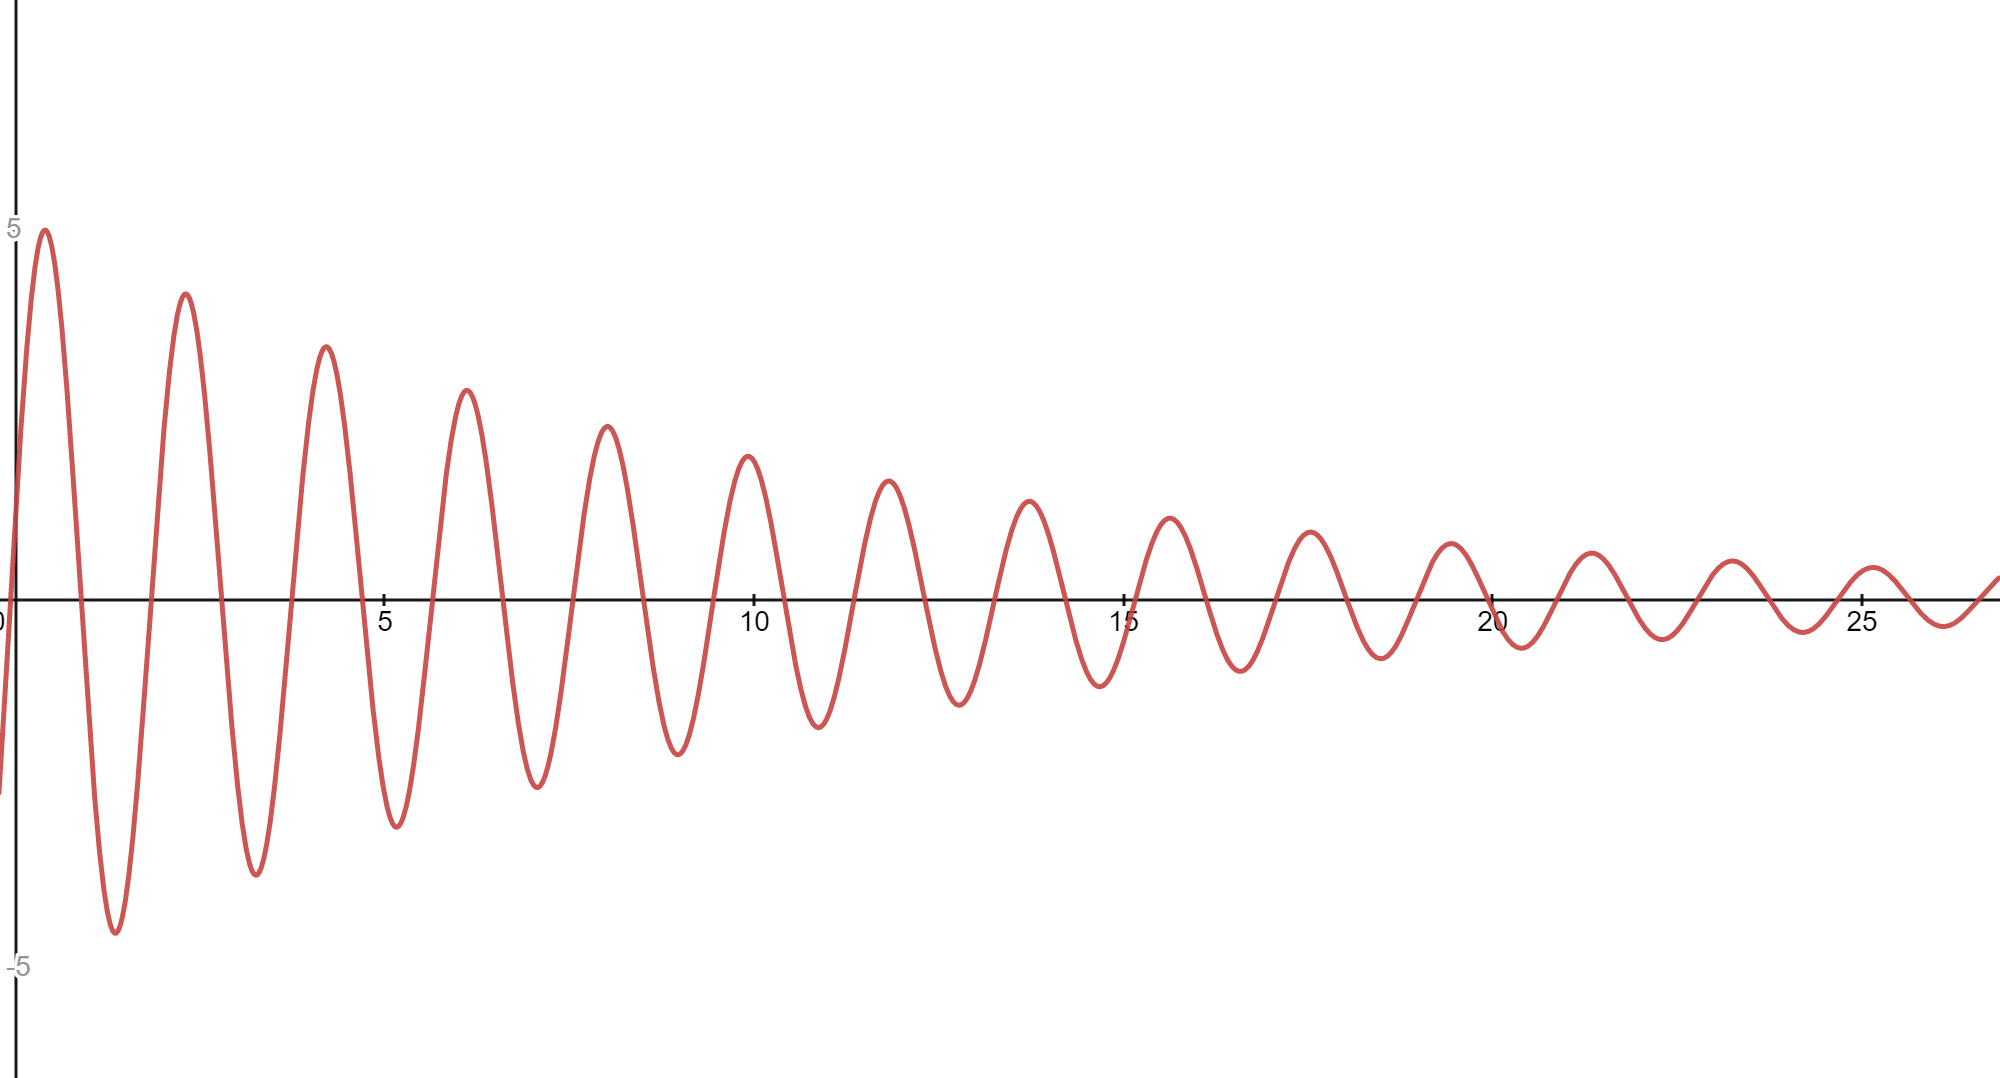
\includegraphics[width=\linewidth]{Oscilatii1.png}
    \caption{$\Delta < 0$}
    \label{fig:oscilatii1}
\end{figure}
\newpage

\section{Rezolvarea numerică a problemei}
\hspace{0.4cm}Metoda pentru metoda lui Euler \cite{kaw10} se bazează pe aproximarea diferențialei, astfel se alege un $\Delta t \approx 0$, care pentru unele date de intrare, nu generează o eroare mare în datele de ieșire. În această lucrare nu ne propunem să demonstrăm regula după care aproximăm diferențiala, ci să observăm cum pentru un anumit pas pentru timp $t$ se modifică valorile funcției $x(t)$ 

\subsection{Metoda lui Euler pentru ecuații diferențiale}
Vom considera ecuația noastră diferențială de mai sus și vom exprima derivata de 2 ori ca funcție de prima derivată și însuți funcția propriu-zisă:
$$\ddot{x}\;=\;f(x,\dot{x})$$

Această rescriere ne conduce la rezolvare următorului sistem de ecuații diferențiale:
\begin{equation}\nonumber
    \left\{
        \begin{array}{lr}
            \dot{x}\;=\;v\\[10pt]
            \dot{v}\;= f(x,\;v)
        \end{array}
    \right.
\end{equation}
\hspace{0.6cm}Dacă considerăm un $\Delta t \approx 0$, putem aproxima derivate astfel:
\begin{equation}\nonumber
        \left\{
        \begin{array}{lr}
            \frac{\Delta x}{\Delta t}\;=\;v\\[10pt]
            \frac{\Delta v}{\Delta t}\;=\;f(x,\;v)
        \end{array}
        \right.
    \end{equation}
\hspace{0.6cm}Ținând cont că $\Delta x\;=\;x_{k+1}\;-\;x_{k}$, obținem următoarele relații:
\begin{equation}\nonumber
        \left\{
        \begin{array}{lr}
            x_{k+1}\;=\;x_k\;+\;v_k\Delta t\\[10pt]
            v_{k+1}\;=\;v_k\;+\;f(x_k, v_k)\Delta t
        \end{array}
        \right.
    \end{equation}
\hspace{0.6cm}În cele ce urmează vom vedea metoda lui Euler în acțiune pentru cazul când $\Delta < 0$, adică rezistența mediului (în cazul nostru aerul) este aproape nesimnificativă, dar cu toate acestea va provoca o funcție extrem de drăguță. Pentru metoda lui Euler vom folosi un pas de $\Delta t = 0,0001$, codul fiind implementat în sistemul de calcul MATLAB.
\newpage
\subsection{Rezolvarea ecuației diferențiale}
\begin{figure}[h]
    \centering
    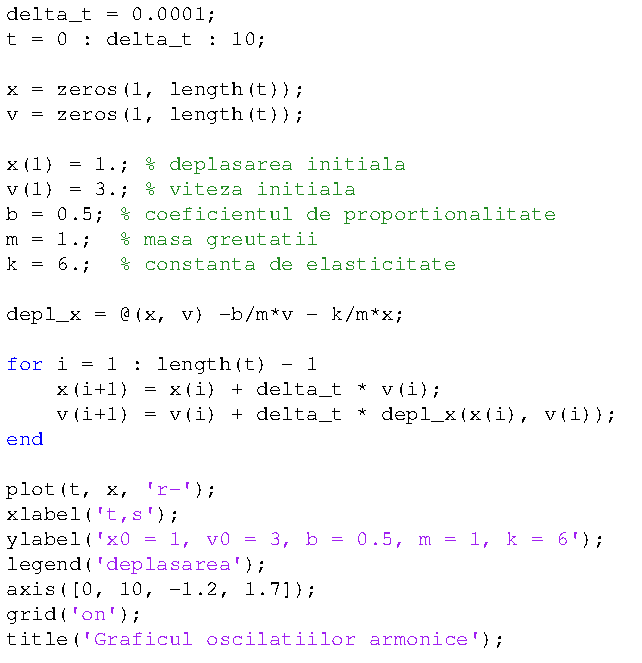
\includegraphics[width=\linewidth, height=\textheight, keepaspectratio]{euler_met}
    \caption{Metoda lui Euler: MATLAB}
    \label{fig:euler}
\end{figure}
Pentru acest mic progrămel vom calcula functia \emph{deplasare} pe intervalul $[0,\;10]$ cu pasul $\Delta t = 0.0001$, apoi vom inițializa datele inițiale și vom calcula componentele principale necesare pentru a putea calcula funcția. Cu ajutorul formulei aflate mai sus.
\newpage
\subsection{Reprezentarea grafică a soluției}
\begin{figure}[h]
    \centering
    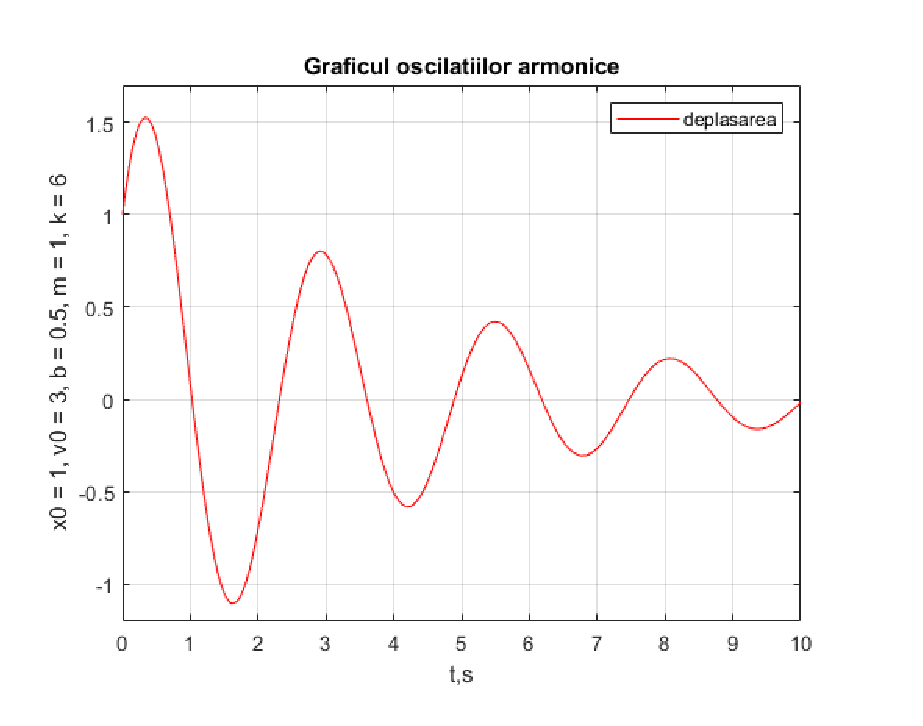
\includegraphics[width=\linewidth, height=\textheight, keepaspectratio]{graph}
    \caption{Metoda lui Euler: Grafic}
    \label{fig:euler_graph}
\end{figure}
\vspace{1cm}
Dacă comparăm Figura \ref{fig:euler_graph} cu Figura \ref{fig:oscilatii1} vom observa că acestea au aceleași forme, clar lucru diferențiază prin valorile inițiale, dar din punct de vedere al analizei matematice acestea sunt identice, în cele ce urmează vom observa diferența în valori dintre metoda analitică și metoda numerică de rezolvare a ecuației diferențiale.
\newpage
\begin{samepage}
\section{Metoda Analitică vs Metoda Numerică}
\hspace{0.5cm}În această secțiune vom prezenta 2 coloane cu date pentru valorile obținute pentru deplasare, cu ajutorul metodei analitice și cu ajutorul metodei numerice. Aceste date sunt generate de MATLAB.

\subsection{Tabelul de valori generate pentru ambele metode}
\begin{center}
    \begin{tabular}{| l | c | c | c | c | c |}
         \hline
         \multicolumn{6}{|c|}{Tabelul de valori pentru funcția deplasare} \\
         \hline
         No. & $V^{i}_T$ & $V^{i}_A$ & $V_T$ & $\Delta V$ & $\epsilon_V$ \\
         \hline
         1 & 1.002697 & 1.002697 & \multirow{20}{*}{8.328047} & \multirow{20}{*}{0.006851} & \multirow{20}{*}{0.082\%}\\
         \cline{1-3}
         2 & 1.408086 & 1.408280 & & &\\
         \cline{1-3}
         3 & 0.077000 & 0.076943 & & &\\
         \cline{1-3}
         4 & -1.049704 & -1.050209 & & &\\
         \cline{1-3}
         5 & -0.699516 & -0.699841 & & &\\
         \cline{1-3}
         6 & 0.391316 & 0.391726 & & &\\
         \cline{1-3}
         7 & 0.783202 & 0.783878 & & &\\
         \cline{1-3}
         8 & 0.172422 & 0.172456 & & &\\
         \cline{1-3}
         9 & -0.504907 & -0.505585 & & &\\
         \cline{1-3}
         10 & -0.441906 & -0.442405 & & &\\
         \cline{1-3}
         11 & 0.123982 & 0.124305 & & &\\
         \cline{1-3}
         12 & 0.419695 & 0.420387 & & &\\
         \cline{1-3}
         13 & 0.159149 & 0.159307 & & &\\
         \cline{1-3}
         14 & -0.229894 & -0.230427 & & &\\
         \cline{1-3}
         15 & -0.264013 & -0.264505 & & &\\
         \cline{1-3}
         16 & 0.018187 & 0.018344 & & &\\
         \cline{1-3}
         17 & 0.216694 & 0.217235 & & &\\
         \cline{1-3}
         18 & 0.117861 & 0.118072 & & &\\
         \cline{1-3}
         19 & -0.096953 & -0.097290 & & &\\
         \cline{1-3}
         20 & -0.150861 & -0.151261 & & &\\
         \hline
    \end{tabular}
\end{center}
\end{samepage}
\newpage
\subsection{Calcularea erorilor valorilor generate}
\hspace{0.4cm}Pentru tabelul de mai sus $V^{i}_T$ reprezintă datele generate după formula aflată analitic (True Values), $V^{i}_A$ reprezintă datele generate după formula aflată numeric (Approximated Values), $V_T$ este valoare medie aboslută a valorilor obținute analitic. $\Delta V$ reprezintă diferența medie dintre fiecare date obținute analitic și numeric, iar în final $\epsilon_V$ este eroarea de calcul a valorilor obținute numeric.

\begin{itemize}
    \item Vom calcula $V_T$ ca o sumă maximizată pentru a nu obține pentru unele cazuri particulare valoarea zero
    $$V_T = \frac{1}{n}\sum_{i=1}^{n} |\;V^{i}_T\;|$$
    \item La fel ca pentru $V_T$ vom calcula $\Delta V$ ca o sumă maximizată la fel ca să nu obținem valoarea zero, fiindcă în datele propuse avem și valori negative
    $$\Delta V = \frac{1}{n}\sum_{i=1}^{n}|\;V_{T}^{i}\;-\;V_{A}^{i}\;|$$
    \item Eroarea $\epsilon_V$ se va calcula așa cum se calculează în liceu, adică raportul dintre eroarea relativă și valoarea medie obținută
    $$\epsilon_V = \frac{\Delta V}{V_T}\;*100\%$$
    \item Pentru $n\;=\;20$ vom obține datele noastre din tabelul de mai sus
\end{itemize}
\section{Concluzia}
\subsection{Analiza datelor și explicarea erorilor}
\hspace{0.4cm}După cum putem observa în tabelul de valori am obținut o eroare de $0.82\%$, pasul pe care l-am folosit pentru aproximarea soluției a fost de $\Delta t = 0.0001$, în limbaj natural acest lucru s-ar traduce că am încercat să facem o aproximare exactă la primele 3 cifre după virgulă și am primit o eroare relativ mică, însă clar lucru pentru unele obiecte de studiu și această eroare este una mare. Deci revenim la concluzia că metoda lui Euler de aproximare a ecuațiilor diferențiale este bună în unele cazuri, din acest motiv există o mulțime de alte metode care fac acelați lucru însă care pentru un anumit set de date lucrează mai bine decât alte metode.

\newpage

\begin{thebibliography}{15}
\bibitem{liu04}
Mingzhu Liu (2004) \emph{Convergence and stability of the semi-implicit Euler method
for a linear stochastic di)erential delay equation}, Elsevier B.V

\bibitem{kaw10}
Autar Kaw (2010) \emph{Euler’s Method for ordinary differential equations}, Luther Madison

\bibitem{altkinson08}
Kendall Atkinson (2008) \emph{Numerical solution of ordinary differential equations}, University of Iowa, Weimin Han, David Stewart

\bibitem{seely00}
A. D., Seely, S (2000) \emph{The Transforms and Applications Handbook: Second Edition}, Ed. Alexander D. Poularikas

\bibitem{murray65}
Murray R. Spiegel, Ph.D. (1965) \emph{Schaum's outline of theory and problems of laplace transforms}, McGraw-Hill. Inc

\bibitem{joel99}
Joel L. Schiff (1999) \emph{The Laplace Transform: Theory and Applications}, Springer

\bibitem{david05}
David Houcque (2005) \emph{Introduction to matlab for engineering students}, Word Inc 

\bibitem{nat01}
Natick M. (2001) \emph{Using Matlab}, The MathWorks Inc

\bibitem{att09}
Stormy Attaway (2009) \emph{Matlab: A Practical Introduction to Programming and Problem Solving
}, Elsevier

\bibitem{chr07}
Christos Xenophontos (2007) \emph{A Beginner’s Guide to MATLAB}, The MathWorks Inc

\bibitem{paul15}
Paul Strode (2015) \emph{Data and Error Analysis in Science A Beginner’s Guide}, Ann Brokaw

\bibitem{georg13}
Georg Fantner (2013) \emph{A brief introduction to error analysis and propagation}, The MathWorks Inc

\bibitem{matt21}
Matthias Hengsberger (2021) \emph{Data and error calculus, PHY112/122 – Praktikum zur Physik I/II}, HS 2020/FS

\bibitem{james2000}
Dr. James E. Parks (2000) \emph{The Simple Pendulum}, James Parks

\bibitem{beatty06}
Millard F. Beatty, Jr (2006) \emph{Principles of Engineering Mechanics, Volume 2, Dynamics- The Analysis of Motion
}, Angelo Miele
\end{thebibliography}
\end{document}
